%
% teil2.tex -- Beispiel-File für teil2 
%
% (c) 2020 Prof Dr Andreas Müller, Hochschule Rapperswil
%
% !TEX root = ../../buch.tex
% !TEX encoding = UTF-8
%
\section{Herleitung der Balkengleichung
	\label{balken:section:teil2}}
\subsection{Variationsprinzip}
Die Variationsrechnung ist ein Teilgebiet der Analysis, das sich mit kleinen Änderungen in Funktionen und Funktionalen beschäftigt, um Minimas und Maximas von Funktionen zu ermitteln.
Dabei handelt es sich um mathematische Ausdrücke, die Integrale über eine unbekannte Funktion und ihre Ableitung darstellen können.
Dabei möchte man ein Maximum, ein Minimum oder einen Sattelpunkt ausfindig machen.

In der Mechanik kommen Variationsrechnungen oft zum Einsatz, sie bilden die Grundlagen alle physikalischen Extremalrechnungen und kommen deshalb in der Mechanik viel zum Einsatz.

\subsection{Minimalprinzip}
Das Minimalprinzip ist ein Konzept, das besagt, dass ein physikalisches System einen bestimmten Zustand annimmt, der mit dem geringsten Input erreicht wird.
In der Physik wird das Minimalprinzip oft formuliert, indem eine minimale Wirkung oder Energie angestrebt wird.

Ein Beispiel hierfür ist eine Feder, die an einem Ende an einer Wand befestigt ist und an ihrem anderen Ende eine Masse trägt.
Wenn man die Masse nach unten zieht und loslässt, bewegt sich die Masse und nimmt eine neue Position ein. In diesem Fall besagt das Minimalprinzip, dass die Masse eine Position einnimmt, bei der die potenzielle Energie möglichst gering ist.

Das Minimalprinzip in Bezug auf die Balkengleichung ist ein grundlegendes Konzept der Mechanik, auch bekannt als das Prinzip von Hamilton.
Es besagt, dass ein System den Gleichgewichtszustand annimmt, bei dem die potenzielle Energie minimal ist.
Für einen Balken tritt dieser Zustand ein, wenn alle äußeren Kräfte, Momente, innere Beanspruchungen sowie Verformungen des Balkens im Gleichgewicht stehen.
Die Anwendung dieses Minimalprinzips führt zur Balkengleichung, die die Gleichgewichtsbedingungen des Balkens beschreibt.

\subsection{Herleitung der Balkengleichung aus dem Variationsprinzip}
Gegeben sind die folgenden Gleichungen, die die Verformungen des Balkens aufgrund der auftretenden Biegespannungen σx beschreibt.
\begin{equation}
	\sigma_x=
	\frac{E}{p}z
\end{equation}
und
\begin{equation}
	\sigma_x=
	\frac{M_y}{EI_y}
\end{equation}
Wenn man diese zwei Gleichungen gleichsetzt, bekommt man
\begin{equation}
	\frac{E}{p}zp
	=\frac{M_y}{EI_y}p
\end{equation}
\begin{equation}
	Ez=
	\frac{M_y}{EI_y}p
\end{equation}
\begin{equation}
	p=
	\frac{EI_y}{M_y}
\end{equation}
\begin{equation}
	\frac{1}{p}=
	\frac{M_y}{EI_y}
\end{equation}
Dabei steht p für den Krümmungsradius

Der Krümmung ergibt sich aus dem Kehrwert der Krümmungsradius.
\begin{equation}
	\frac{1}{p}=
	\frac{M_y}{EI_y}=
	\kappa
\end{equation}

Bei Biegungen, die aufgrund von Querkräfte auftreten, ist das Moment veränderlich.
Das Moment hängt von der Position x ab und ist daher nicht konstant.
Liegt also eine Querkraftbiegung vor, so ergibt sich ein anderer Moment für jeden Schnitt.
Dies führt dazu, dass die Krümmung des Balkens bzw. Biegelinie von der Position x abhängt.
\begin{figure}
\begin{center}
	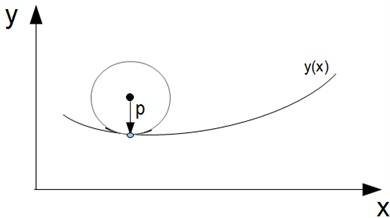
\includegraphics[width=0.8\textwidth]{papers/balken/images/teil2/BiegungBalke1.jpg}
\end{center}
\caption{Darstellung der Biegelinie y(x) mit den Krümmungsradius p.}
\end{figure}
Um die Krümmung zu bestimmen, benötigen wir den kürzesten Weg zwischen beiden Auflagern des Balkens.
Dabei bezeichnen wir die beiden Auflagern als die Punkte $(x_1, y_1)$ und $(x_2, y_2)$ in der $x$-$y$-Ebene, wobei $x_1 \ne x_2$.
\begin{figure}
\begin{center}
	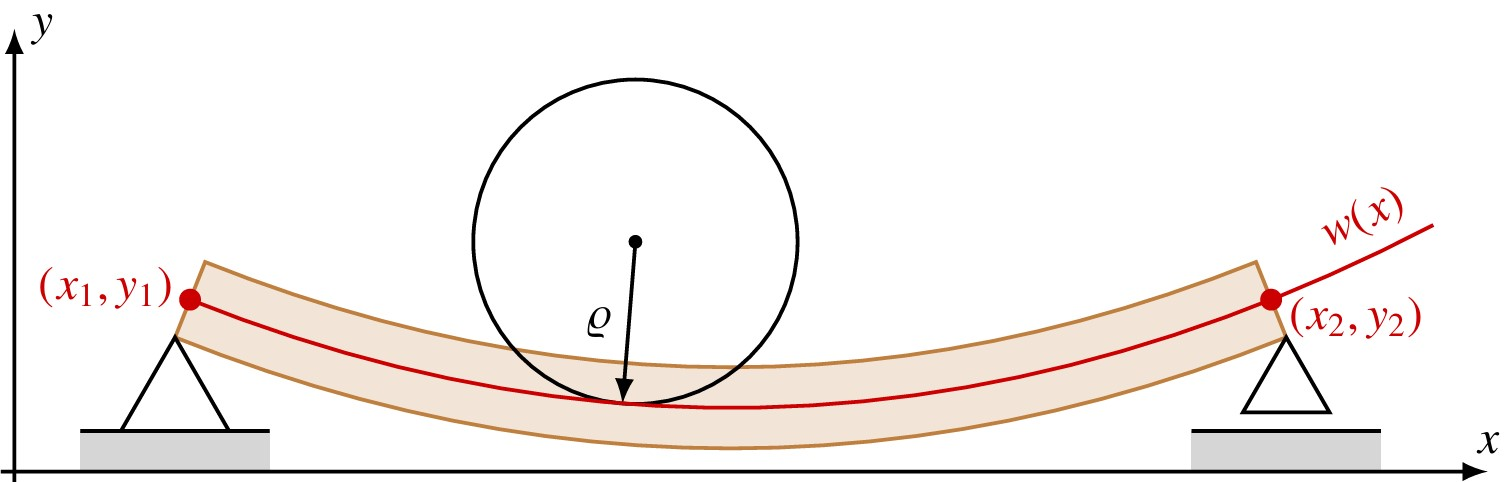
\includegraphics[width=0.8\textwidth]{papers/balken/images/teil2/BiegungBalke2.jpg}
\end{center}
\caption{Darstellung der Biegelinie y(x) mit der Balke (blau gezeichnet) und deren Auflagern.}
\end{figure}
Um die Länge dieser Kurve in der x-y-Ebene zu berechnen, berechnen wir zuerst der Länge einer Gerade auf der Kurve y(x)
\begin{equation}
	\Delta s=
	\sqrt{\Delta x^2+\Delta y^2}\approx\sqrt{1+y'(x)^2}\cdot\Delta x
\end{equation}
Daraus rechnen wir mit dem Integral die Kurvenlänge.
\begin{equation}
	l(y)=
	\int_{x_1}^{x_2}\sqrt{1+{y'(x)}^2}dx
\end{equation}
Unsere Langrange-Funktion ist somit:
\begin{equation}
	L(x,y,y')=
	\sqrt{1+{y'}^2}
\end{equation}
Mittels der partiellen Ableitung von L, erhalten wir die folgende.
\begin{equation}
	\frac{\partial L}{\partial y}=
	0
\end{equation}
\begin{equation}
	\frac{\partial L}{\partial y'}=
	\frac{2y'}{2\sqrt{1+{y'}^2}}=
	\frac{y'}{\sqrt{1+{y'}^2}}
\end{equation}
Jetzt setzen wir y(x) ein und leiten nach x ab.
\begin{equation}
	\frac{d}{dx}\frac{\partial L}{\partial y'}(x,y(x),y'(x))=
	\frac{d}{dx}\frac{y'(x)}{\sqrt{1+{y'}^2}}=
	\frac{y''(x)\sqrt{1+{y'}^2}-y'(x)\left(\frac{y'(x)}{\sqrt{1+{y'}^2}}\right)y''(x)}{1+{y'(x)}^2}
\end{equation}
\begin{equation}
	\frac{d}{dx}\ \frac{\partial L}{\partial y'}(x,y(x),y'(x))=
	\frac{(1+{y'(x)}^2-{y'(x)}^2)y''(x)}{\left(1+{y'}^2\right)^\frac{3}{2}}=
	\frac{y''}{\left(1+{y'}^2\right)^\frac{3}{2}}
\end{equation}
Dabei erhalten wir die Gleichung.
\begin{equation}
	\kappa=
	\frac{1}{p}=
	\pm\frac{y''}{\left(1+{y'}^2\right)^\frac{3}{2}}
\end{equation}
Da wir in unserem Fall w(x) als Funktion für die Biegelinie verwenden, müssen wir das Vorzeichen noch bestimmen.
Da ein positives Moment eine Biegung nach unten verursacht, müssen wir ein negatives Vorzeichen verwenden. Dabei erhalten wir.
\begin{equation}
	\kappa=
	\frac{1}{p}=
	-\frac{w''}{\left(1+{w'}^2\right)^\frac{3}{2}}
\end{equation}
mit
\begin{equation}
	w'=
	\frac{dy}{dx} 
\end{equation}
und
\begin{equation}
	w''=
	\frac{d^2y}{dx^2}
\end{equation}

w = Funktion der Durchbiegung

w’ = Neigung der Durchbiegung

w’’ = Krümmung

Da wir in der Baustatik den Rechtssystem verwenden, kehren wir den z-Achse so, dass nach unten das positive Vorzeichen ist

\begin{figure}
\begin{center}
	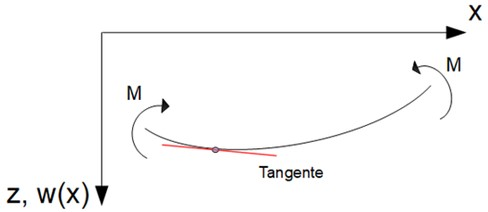
\includegraphics[width=0.8\textwidth]{papers/balken/images/teil2/BiegungverdrehteAchsen.jpg}
\end{center}
\caption{Abbildung von den verdrehten z-Achse und die positive Momenten, welche auf der Biegelinie wirken.}
\end{figure}
Unsere Funktion zeigt eine Krümmung nach links, jedoch durch die Spiegelung an der z-Achse ergibt sich eine Krümmung nach rechts.
Bei Rechtskrümmungen sind die 2. Ableitungen kleiner als 0. w’’ < 0.
Das ergibt.
\begin{equation}
	\kappa=
	-\frac{w''}{\left(1+{w'}^2\right)^\frac{3}{2}}=
	\frac{M_y}{EI_y}
\end{equation}
Der Term w’ kann vernachlässigt werden, da im Betracht des Hookesche Gesetz nur kleine Verformungen vorliegen.
Daraus ergeben sich Tangentensteigungen von w’ << 1.
\begin{equation}
	\kappa=
	-\frac{w''}{\left(1+{w'}^2\right)^\frac{3}{2}}=
	-\frac{w''}{\left(1+0\right)^\frac{3}{2}}=
	-\frac{w''}{1}=-w''=
	\frac{M_y}{EI_y}
\end{equation}
Daraus ergibt sich.
\begin{equation}
	w''=
	-\frac{M_y}{EI_y}
\end{equation}
mit
\begin{equation}
	\kappa=
	-w''
\end{equation}
Temperaturunterschiede verursachen Verformungen in der Balkenachse.
Daher ist es wichtig, die Krümmung der Biegelinie bei Temperaturänderungen zu berücksichtigen.
Daraus ergibt sich der Formel.
\begin{equation}
	w''=
	-\frac{M_y}{EI_y}-\alpha_{th}\frac{\Delta T}{h}
\end{equation}

αth = thermische Ausdehnungskoeffizient des Balkenmaterials

ΔT = Temperaturunterschied

h = Höhe des Balkens

Iy = Flächenträgheitsmoment

Den oben genannten Formel kann auch folgend angegeben werden.
\begin{equation}
	w''''=
	\left(-\frac{M_y}{EI_y}-\alpha_{th}\frac{\Delta T}{h}\right)^{''}
\end{equation}
Bei einer linearen Temperaturverlauf ergibt sich bei der zweiten Ableitung 0.
\begin{equation}
	w''''=
	\left(-\frac{M_y}{EI_y}\right)^{''}
\end{equation}
Die erste Ableitung des Biegemoments ergibt die Querkraft.
\begin{equation}
	\frac{dM}{dx}=
	M'=
	Q
\end{equation}
Daraus ergibt sich.
\begin{equation}
	w'''=
	-\frac{Q}{(EI_y)'}
\end{equation}
Mit konstanter Biegesteifigkeit EI = konst. erfolgt.
\begin{equation}
	EIw^{'''}=
	-Q\left(x\right)
\end{equation}
Die 1. Ableitung der Querkraft bzw. die 2, Ableitung des Biegemoments ergibt der Linienlast entlang der x-Achse.
\begin{equation}
	\frac{dQ}{dx}=
	Q'=
	-q(x)
\end{equation}
\begin{equation}
	w''''=
	\frac{-q(x)}{(EI_y)''}
\end{equation}
Mittels dieser Formel kann die Biegelinie w(x) ermittelt werden
\begin{equation}
	EIw^{''''}=
	q\left(x\right) 
\end{equation}
Jetzt Integrieren wir die Formel viermal.

1. Integration (Querkraft)
\begin{equation}
	EIw^{'''}=
	\int q_0dx=
	q_0\cdot x+C_1
\end{equation}
2. Integration (Biegemoment)
\begin{equation}
	EIw''=
	\int{q_0\cdot x}dx+\int C_1dx=
	\frac{1}{2}q_0x^2+C_1x+C_2
\end{equation}
3. Integration
\begin{equation}
	EIw'=
	\int{\frac{1}{2}q_0x^2}dx+\int{C_1x}dx+\int C_2dx=
	\frac{1}{6}q_0x^3+\frac{1}{2}C_1x^2+C_2x+C_3
\end{equation}
4. Integration
\begin{equation}
	EIw=
	\int{\frac{1}{6}q_0x^3}dx+\int{\frac{1}{2}C_1x^2}dx+\int{C_2x}dx+\int C_3=
	\frac{1}{24}q_0x^4+\frac{1}{6}C_1x^3+\frac{1}{2}C_2x^2+C_3x+C_4
\end{equation}
Jetzt werden die Randbedingungen berücksichtigt.
In unserem Fall haben wir bei (x1, y1) einen Festlager und bei (x2, y2) ein Loslager.
Dabei gelten für den Fest- und Loslager w = 0 und M = 0, das bedeutet, dass an diese Stellen keine Verschiebung in z-Richtung stattfindet und dass keinen Momenten aufgenommen werden können.

Es gilt.
\begin{equation}
	EIw'' =
	-M_y
\end{equation}
und
\begin{equation}
	EIw'''=
	-Q_z
\end{equation}
Als erstes betrachten wir die Stelle $(x_1, y_1)$ mit den Festlager.
Dabei setzen wir den Ursprung unser Koordinatennetz bei $(x_1, y_1)$, damit ergibt sich x = 0.
Die Bedingungen sind: w = 0 und M = 0.
\begin{equation}
	EIw=
	\frac{1}{24}q_0x^4+\frac{1}{6}C_1x^3+\frac{1}{2}C_2x^2+C_3x+C_4
\end{equation}
w = 0 und x = 0 einsetzen:
\begin{equation}
	EI\cdot0=
	\frac{1}{24}q_00^4+\frac{1}{6}C_10^3+\frac{1}{2}C_20^2+C_30+C_4
\end{equation}
\begin{equation}
	C_4=
	0
\end{equation}
Für den Momentenberechnung nehmen wir die 2. Ableitung und setzen M = 0 ein
\begin{equation}
	EIw''=
	-M_y=
	\frac{1}{2}q_0x^2+C_1x+C_2
\end{equation}
\begin{equation}
	0=
	\frac{1}{2}q_00^2+C_10+C_2
\end{equation}
\begin{equation}
	C_2=
	0
\end{equation}
Jetzt machen wir die gleichen Berechnungen an der Stelle $(x_2, y_2)$ mit den Loslager, für $x_2$ setzen wir L (für der Länge des Balkens) ein.
\begin{equation}
	EIw=
	\frac{1}{24}q_0x^4+\frac{1}{6}C_1x^3+\frac{1}{2}C_2x^2+C_3x+C_4
\end{equation}
w = 0 und x = L, sowie $C_2$ = 0 und $C_4$ = 0 werden eingesetzt.
\begin{equation}
	EI\cdot0=
	\frac{1}{24}q_0L^4+\frac{1}{6}C_1L^3+\frac{1}{2}0\cdot L^2+C_3L+0
\end{equation}
\begin{equation}
	0=
	\frac{1}{24}q_0L^4+\frac{1}{6}C_1L^3+C_3L
\end{equation}
\begin{equation}
	C_3=
	-\frac{1}{24}q_0L^3-\frac{1}{6}C_1L^2
\end{equation}
Für den Momentenberechnung nehmen wir die 2. Ableitung und setzen M = 0, x = L und $C_2$ = 0 ein.
\begin{equation}
	EIw''=
	-M_y=\frac{1}{2}q_0x^2+C_1x+C_2
\end{equation}
\begin{equation}
	0=
	\frac{1}{2}q_0L^2+C_1L+0
\end{equation}
\begin{equation}
	C_1=
	-\frac{1}{2}q_0L
\end{equation}
$C_1$ in $C_3$ einsetzen:
\begin{equation}
	C_1=
	-\frac{1}{2}q_0L
\end{equation}
\begin{equation}
	C_3=
	-\frac{1}{24}q_0L^3-\frac{1}{6}C_1L^2
\end{equation}
\begin{equation}
	C_3=
	-\frac{1}{24}q_0L^3-\frac{1}{6}\left(-\frac{1}{2}q_0L\right)L^2
\end{equation}
\begin{equation}
	C_3=
	-\frac{1}{24}q_0L^3+\frac{1}{12}q_0L^3
\end{equation}
\begin{equation}
	C_3=
	\frac{1}{24}q_0L^3
\end{equation}
Die Konstanten werden in die Biegelinien-Gleichung eingesetzt.
\begin{equation}
	EIw=
	\frac{1}{24}q_0x^4+\frac{1}{6}\left(-\frac{1}{2}q_0L\right)x^3+\frac{1}{2}\cdot0\cdot x^2+\left(\frac{1}{24}q_0L^3\right)x+0
\end{equation}
\begin{equation}
	EIw=
	\frac{1}{24}q_0x^4+\frac{1}{6}\left(-\frac{1}{2}q_0L\right)x^3+\left(\frac{1}{24}q_0L^3\right)x
\end{equation}
\begin{equation}
	EIw=
	\frac{1}{24}q_0x^4-\frac{1}{12}q_0Lx^3+\frac{1}{24}q_0L^3x
\end{equation}
\begin{equation}
	EIw=
	\frac{1}{12}q_0\left(\frac{1}{2}x^4-Lx^3+\frac{1}{2}L^3x\right)
\end{equation}
\begin{equation}
	w=
	\frac{1}{12EI}q_0\left(\frac{1}{2}x^4-Lx^3+\frac{1}{2}L^3x\right)
\end{equation}

\subsection{Herleitung der Balkengleichung aus dem Baustatik}
Die Herleitung der Balkengleichung lässt sich ebenso gut mit den konventionellen Methoden der Baustatik durchführen, indem man die Beziehung zwischen dem Biegemoment M und der Biegung w verwendet
\begin{figure}
\begin{center}
	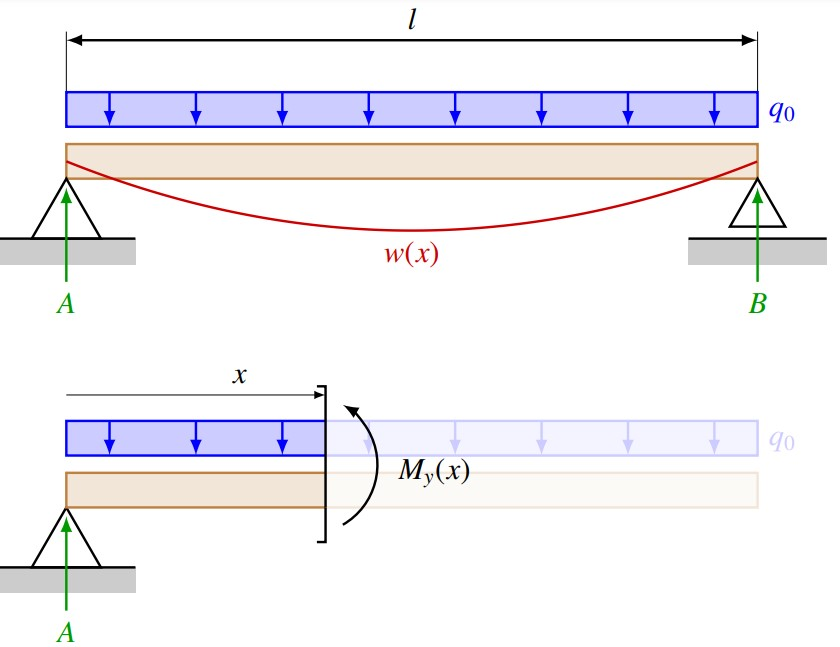
\includegraphics[width=0.8\textwidth]{papers/balken/images/teil2/HerleitungBaustatik.jpg}
\end{center}
\caption{Darstellung unsere Balke mit den Auflagern A und B und der Linienlast q0.}
\end{figure}
Gegeben ist:
\begin{equation}
	w''(x)=
	-\frac{M_y(x)}{EI_y}
	\rightarrow-M_y(x)=
	EI_y\cdot w''(x)
\end{equation}
Zuerst berechnen wir die Auflagerkräfte A und B.
\begin{equation}
	A=
	B=
	\frac{q_0\cdot L}{2}
\end{equation}
Danach berechnen wir den Schnittmoment an der Stelle x.
Moment ist gleich Kraft mal Hebelarm.
\begin{equation}
	M_y(x)=
	A\cdot x-\frac{q_0\cdot x^2}{2}=
	\frac{q_0\cdot L}{2}\cdot x-\frac{q_0\cdot x^2}{2}
\end{equation}
Jetzt setzen wir $My(x) = EIy \cdot w''(x)$ ein
\begin{equation}
	EI_y\cdot w''(x)=
	\frac{q_0\cdot x^2}{2}-\frac{q_0\cdot L}{2}\cdot x
\end{equation}
\begin{equation}
	EI_y\cdot w'\left(x\right)=
	\frac{q_0}{2}\cdot\frac{1}{3}\cdot x^3-\frac{q_0\cdot L}{2}\cdot\frac{1}{2}\cdot x^2+C_1
\end{equation}
\begin{equation}
	EI_y\cdot w\left(x\right)=
	\frac{q_0}{6}\cdot\frac{1}{4}\cdot x^4-\frac{q_0\cdot L}{4}\cdot\frac{1}{3}\cdot x^3+C_1\cdot x+C_2
\end{equation}
\begin{equation}
	EI_y\cdot w\left(x\right)=
	\frac{q_0}{24}\cdot x^4-\frac{q_0\cdot L}{12}\cdot x^3+C_1\cdot x+C_2
\end{equation}
1. Randbedingung: Durchbiegung an der Stelle x = 0 ist 0.
\begin{equation}
	EI_y\cdot w\left(x\right)=
	\frac{q_0}{24}\cdot x^4-\frac{q_0\cdot L}{12}\cdot x^3+C_1\cdot x+C_2
\end{equation}
\begin{equation}
	0=
	\frac{q_0}{24}\cdot0^4-\frac{q_0\cdot L}{12}\cdot0^3+C_1\cdot0+C_2
\end{equation}
\begin{equation}
	C_2=0
\end{equation}
2. Randbedingung: Durchbiegung an der Stelle x = L ist auch 0.
\begin{equation}
	EI_y\cdot w\left(x\right)=
	\frac{q_0}{24}\cdot x^4-\frac{q_0\cdot L}{12}\cdot x^3+C_1\cdot x+C_2
\end{equation}
\begin{equation}
	0=
	\frac{q_0}{24}\cdot L^4-\frac{q_0\cdot L}{12}\cdot L^3+C_1\cdot L+0
\end{equation}
\begin{equation}
	C_1=
	\frac{q_0\cdot L^3}{24}
\end{equation}
Daraus ergibt sich der Formel:
\begin{equation}
	EI_y\cdot w\left(x\right)=
	\frac{q_0}{24}\cdot x^4-\frac{q_0\cdot L}{12}\cdot x^3+\frac{q_0\cdot L^3}{24}\cdot x
\end{equation}
\begin{equation}
	w=
	\frac{1}{12EI_y}q_0\left(\frac{1}{2}x^4-Lx^3+\frac{1}{2}L^3x\right)
\end{equation}
Das ist äquivalent zu dem, was wir bei der mathematischen Herleitung erhalten haben.

\subsection{Erläuterung der Annahmen und Randbedingungen}
Um die Berechnungen innerhalb der Plattentheorie pragmatischer zu gestalten, werden einige Vereinfachungen vorgenommen und die Randbedingungen festgelegt, unter denen sie gültig sind.
Dadurch können die Berechnungen vereinfacht und lösbar gemacht werden.
Zu den Annahmen und Randbedingungen gehören folgende Aspekte:

\begin{enumerate}
	\item Die Balken werden als dünn angenommen, die hat zu bedeuten, dass die Dicke im Vergleich zur Länge des Balkens vernachlässigbar klein ist und deshalb für die Berechnung irrelevant ist.
	\item Die Balken sind eine konstante Linienlast ausgesetzt.
	\item Die Balken werden als ebene Struktur betrachtet, ohne signifikante Krümmungen und Verwindungen.
	\item Im unbelasteten Zustand bleiben Linienabschnitte, die senkrecht zur Mittelfläche stehen, auch im verformten Zustand gerade und senkrecht zur verformten Mittelfläche
	\item Randbedingungen werden festgelegt, wobei die Art der Auflagerung oder Einspannung des Balkens berücksichtigt wird.
	Diese Randbedingungen sind in der untenstehenden Tabelle aufgeführt.
	\item Die Verformungen und Spannungen innerhalb des Balkens werden als vernachlässigbar klein betrachtet und können deshalb ausgeschlossen werden
	\item Die Biegesteifigkeit des Balkens ist als konstant anzunehmen
	\item Es wird angenommen, dass die Temperaturdifferenz, die zu Verformungen der Balkenachse führt, konstant ist, und daher ergibt seine zweite Ableitung Null.
	\item Die Belastungen des Balkens wirken senkrecht zur Achse.
\end{enumerate}
\begin{figure}
\begin{center}
	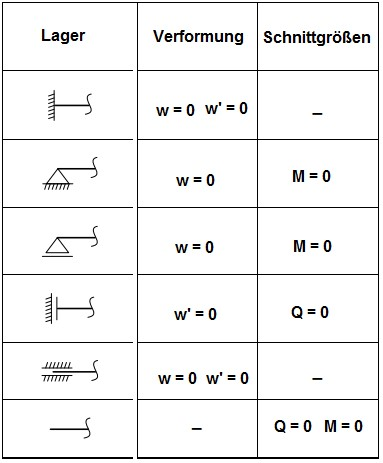
\includegraphics[width=0.8\textwidth]{papers/balken/images/teil2/Randbedingungen.jpg}
\end{center}
\caption{Tabelle der unterschiedlichen Randbedingungen für verschiedene Auflagertypen.}
\end{figure}
